\section{Final Design}


\subsection{System overview}
\label{system-overview}

\figref{system-diagram} shows the high-level system interactions of the components used in our project.
The components we built are shown in solid rectangles.

The finished project consists of three main parts: The overlay FPGA, bitstream generation software, and interfacing of inputs/outputs of the overlay FPGA.

The \emph{Overlay FPGA} is a Verilog HDL circuit implementation of the Academic FPGA model which is constructed as an overlay on a Xilinx FPGA board.
The arrangement, size and connectivity of the overlay circuit is controllable via parameters in the source Verilog.
The overlay FPGA consists of organized tiles of \emph{logic block}, \emph{connection block}, and \emph{switch block} modules.
Together, these modules allow the overlay FPGA to implement different logic circuits.

\begin{figure}[!h]
	\centering
	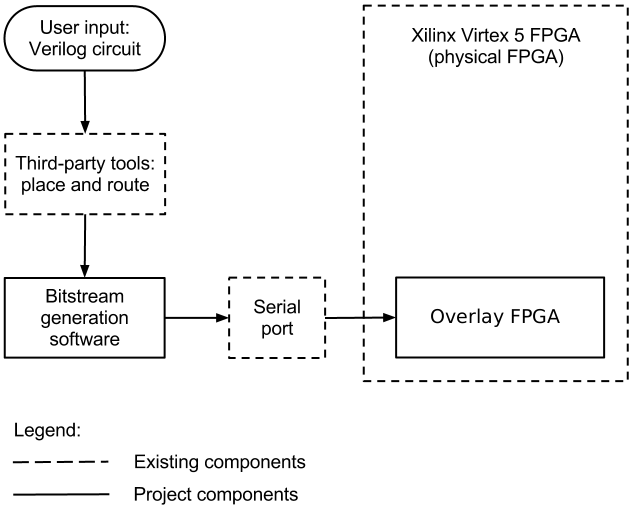
\includegraphics[scale=0.6]{system.png}
	\caption{System overview}
	\label{system-diagram}
\end{figure}

The \overlay can be configured to implement user-specified \emph{test circuits} that have been placed and routed by VPR.
This is achieved using the \emph{bitstream generation and programming software} that translates the VPR output circuit into a bitstream that the overlay FPGA understands.
The bitstream is then injected into the overlay FPGA via a \emph{serial interface}.
The FPGA receives and decode the bitstream into the appropriate test circuits on the overlay.

Finally, the circuits on the overlay FPGA are controlled by connecting devices such as switches and LEDs connected through the physical FPGA.



\subsection{Module design}

The \emph{Overlay FPGA} is composed of a two-dimensional array of \emph{Logic tiles}.
The logic tiles make it easier to build a large overlay, and help keep the internal 
logic modules organized.
Each logic tile consists of one \emph{logic block module}, two \emph{connection block modules}, 
and one \emph{switch block module}.
\figref{tile-diagram} shows the internal composition of a single logic tile.

\begin{figure}[!h]
	\centering
	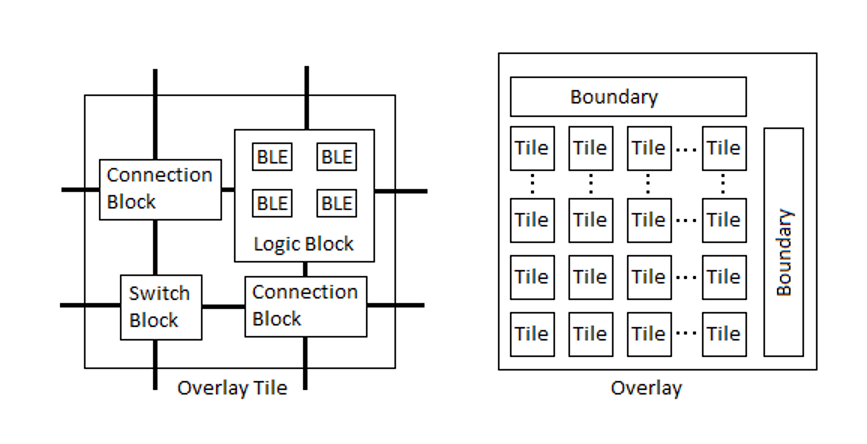
\includegraphics[scale=0.7]{overlay.png}
	\caption{Logic tile and tile arrangement}
	\label{tile-diagram}
\end{figure}

The \emph{Logic block module} consists of programmable look-up tables that perform all of the logical 
functionality required by the circuit.
A logic block module may be composed of multiple look-up tables, the number of which 
can be determined by Verilog parameters.

The \emph{Connection block} and \emph{Switch block} modules regulate the routing of signals in the overlay.
\emph{Connection blocks} connect logic block signals to buses that run throughout the 
overlay.
\emph{Switch blocks} control the routing between buses when they cross each other.

\begin{figure}[!h]
	\centering
	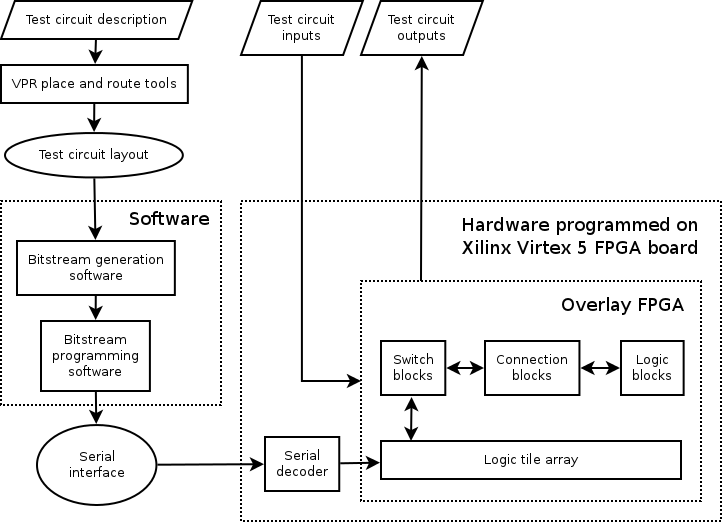
\includegraphics[scale=0.6]{modules.png}
	\caption{Module overview}
	\label{module-diagram}
\end{figure}

\figref{module-diagram} shows the relationship between the higher-level modules.

The \emph{Bitstream generation software} is a program that translates VPR output circuits into a bitstream capable of programming the overlay FPGA directly.
The program consists of functions that parse the output from VPR and generate the 
appropriate bitstream from the parsed information.

The \emph{Bitstream programming software} takes the bitstream formed by the bitstream generator and formats it for proper transmission over a serial interface.

The \emph{Serial decoder} is a circuit attached to the overlay FPGA that receives the 
bitstream sent through the serial interface.
It decodes and extracts the bitstream from the serial format, then injects it into the overlay circuit to configure the overlay.



\subsection{Assessment of design}

The decision to take advantage of the custom 32-bit shift registers in implementing our design entails the following trade-offs versus using only basic Verilog logic:
\begin{itemlist}
	\item The design is more efficient area and timing-wise.
	\item The data describing the circuit (known as the \emph{bitstream}) which is needed to program the design is larger.
	\item The maximum size of the design is limited by the amount of 32-bit shift registers available on the FPGA board, as opposed to the amount of flops.
	\item The design is incompatible with boards that do not have custom 32-bit shift registers.
\end{itemlist}

We have decided that performance efficiency outweighs the negative aspects of the larger bitstream and limitation of implementation platforms.
If the design is successful, adaptations can be made in the future to support the implementation of the design on more FPGA boards.

We have also looked into using a Clos network for the logic block crossbar.
Currently, the crossbar is implemented using layered multiplexers built from 32-bit shift registers for each lookup table input, and is the most resource-heavy part of the tile.
By replacing all the input multiplexers with a large Clos network, it is possible to reduce the number of shift registers consumed by up to 35\%.
However, the fact that we only have 32-bit shift registers available as building blocks severely restricts the size of the crossbar, and would have removed the flexibility of choosing the number of logic block inputs currently built into the design.
Additionally, the algorithm for routing the Clos network is much more complex than the current crossbar design; the signal path to each lookup table input are dependent on each other, and cannot be routed individually.
There are existing algorithms for routing Clos networks, but they focus on networks where one input can only route to one output.
For our design, we need a network that can route multiple outputs from a single input.
We were unable to develop our own algorithm for the Clos network due to time constraints.
Because of these reasons, we decided against incorporating Clos networks into our current design.
For future improvements, we may return to Clos networks.


